\documentclass[11pt]{article}

\usepackage[utf8]{inputenc}
\usepackage{geometry}
\geometry{a4paper, margin=1in}
\usepackage{graphicx}
\usepackage{hyperref}
\usepackage{fancyhdr}

\setlength{\headheight}{15pt}
\pagestyle{fancy}
\fancyhf{}
\rhead{Computer Workshop Course}
\lhead{Final Assignment}
\rfoot{Page \thepage}

\title{Final Assignment}
\author{Mani Zamani}
\date{January 2025}

\begin{document}

\maketitle
\newpage
\tableofcontents
\newpage

\section{repository link}
\paragraph{\url{https://github.com/Manizmn84/FinalAssignment}}

\section{Git and GitHub}
\subsection{Repository Initialization and Commits}

Write about how you set up the repository for this assignment. Explain every
 step in detail?

\paragraph{To set up a repository, first of all, we must have a GitHub account. After creating a GitHub account or logging into the account, we perform the following steps:}

\begin{itemize}
    \item Go to the repository section in your account
    \item Click on New Repository
    \item Enter the explanation in the description field
    \item Choose whether the repository is public or private
    \item Choose "add README"
    \item Click on create repository 
\end{itemize}

\subsection{GitHub Actions for LaTeX Compilation}
Provide a walkthrough of setting up GitHub Actions to automatically compile
 your LaTeX document and any challenges you encountered?\newline

\noindent{To launch a compiler for LaTeX with GitHub actions, you must set up a workflow and enter your codes for compilation in the `main.yml` file. It didn't work with tags on my system, so I had to go with push. One of the challenges I faced was that when I wanted to do it with tags, it wouldn't work, and I had to proceed with a push mode.}

\section{Exploration Tasks}
\subsection{Vim Advanced Features}
\paragraph{Explore and document 3 advanced features of Vim that were not covered in class:}

\begin{enumerate}
    \item One of Vim’s features is macros, with the help of which you can record a sequence
 of keystrokes that can be executed with only one keystroke. The reason for using
 this feature is clear from the fact that in text editing and in programming, some
 tasks need to be executed over and over again. We can call this task repetitive
 tasks, for example, we can refer to formatting code or generating boilerplate text.
    \item Vim’s another feature is a tabbed interface which allows you to open many files and
 switch between them easily .this can be usefull to save your time while you working.
 Tabs support multiple windows, making it easy to work with multiple files in same
 time.
    \item last feature is the folding, which is provided for programmers and some people who
 work with huge documents, this feature allows you to fold and unfold sections of
 text, making it easy to navigate and work with large files.this feature is useful for
 saving time and no need to spend time to transport in large documents.
\end{enumerate}

\subsection{Memory profiling}
\subsubsection{Memory Leak}
\noindent{\small A memory leak occurs when a programmer allocates memory but fails to free it. f we don’t free the allocated memory, the possibility of memory leak is high}

\subsubsection{Memory profilers}
\noindent{\small valgrind is amazing tool witch is use for identification allocated memory.if we
 allocate a part of memory and we did not free it in purpose and then we open
 this application we will see that it has tell us about the allocated memory and
 free memory and the size of memory witch is allocated.}

\subsection{GNU Linux Bash Scripting}
\subsubsection{fzf}
\noindent{\small Fuzzy search is a search algorithm that allows users to ignore minor errors, such as misspellings, in one or a few letters of a word.\newline}
\noindent{\small To install `fzf` and understand the command: \texttt{ls | fzf}, this command helps you navigate and select files or directories using fuzzy search. The `ls` command lists the files, and with `fzf`, you can quickly search through them.}

\subsubsection{Using fzf to find your favorite PDF}
\noindent{\small First of all, we have to install `fd`. Then we can use this command to list all PDF files in that repository: \texttt{fd -e pdf}. However, there is a problem with this command as it lists only the PDF files in the current directory. A better command is \texttt{fd -t -e pdf}, which can list all PDF files from the current directory and any subdirectory. After listing the PDF files, we know the name of the PDF that we want to select, and we use this command to select it: \texttt{fd -t pdf -E '.*' file name | fzf}. In this command, \texttt{-t} is for recursively searching, \texttt{-E '.*'} is used to refer to PDF files, and \texttt{fzf} helps in selecting the desired file.}


\subsubsection{Opening the file using Zathura}
\noindent{\small To open the selected file in Zathura, use the command: \texttt{fd -t pdf -E '.*' | fzf \&\& zathura (\$cat -)}. The \texttt{cat -} command passes stdin to Zathura, allowing it to open and display the selected file.}


\section{Git and FOSS}
\subsection{README.md}
\noindent{write in README.md file}


\subsection{Issues}
\begin{figure}[h]
    \centering
    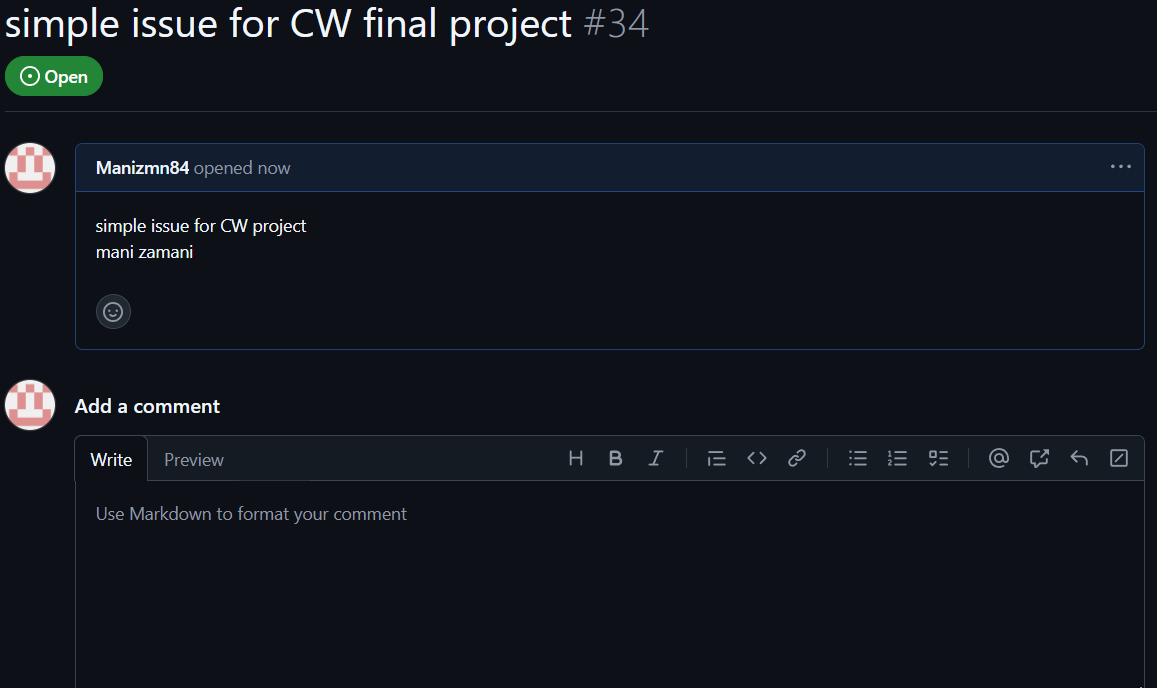
\includegraphics[width=0.5\textwidth]{issue.png}
    \caption{simple issue}
\end{figure}


\subsection{FOSS contribution}
\paragraph{Do you see yourself contributing to FOSS projects in the future? If yes, what kind of
 projects are you interested in contributing to? If no, why not?\newline}

\noindent Yes, I see myself contributing to FOSS projects in the future. I believe that for someone like me, who has no experience with large-scale projects, participating in open-source projects can be a great opportunity to gain valuable experience and develop my skills. Contributing to these projects will allow me to learn from real-world codebases and collaborate with other developers, which will help me grow professionally.

\end{document}